%!TeX root = ../complex_net_report_senacheribbe.tex
\graphicspath{{../assignment1/figures/}}

\subsection{Introduction}

In this first assignment, we evaluate the centrality of the nodes in a medium size graph (some thousands of nodes), using different centralities measures.\\
The graph chosen for the following analysis is a protein-protein interaction (PPI) graph in Homo Sapiens (taken from \cite{db_react}). The nodes represents proteins and two nodes are connected by an edge if they have some kind of interaction.\\
The centralities in protein-protein interaction networks are a powerful tool to understand which proteins play an important role and are essential for the organism.

\subsection{Graph properties}
First of all, the graph is read from file and processed to remove self-loops and extract only the largest connected component.
The resulting graph has  $n = 5973$ vertices and $m = 145778$ edges. It is stored by employing its adjacency matrix represented in sparse matrix format.
The structure of the matrix is shown in the sparsity plot of \cref{fig:1_sparsity}.

\begin{figure} [!ht]
	\centering
	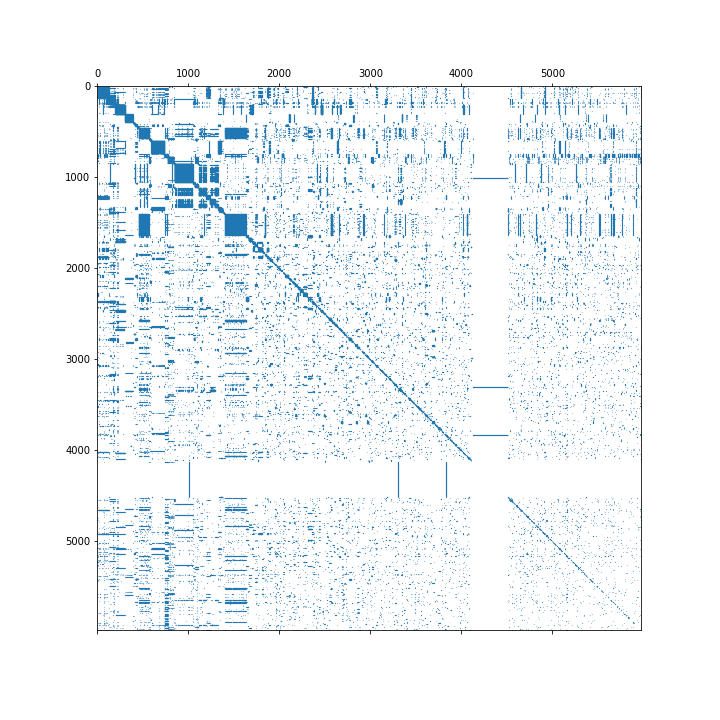
\includegraphics[width=.5\linewidth, clip, trim={2cm 2cm 2cm 2cm}]{sparsity}
	\caption{Sparsity of PPI graph with  $n = 5973$ and $m = 145778$}
	\label{fig:1_sparsity}
\end{figure}
For completeness we also report in  \cref{fig:1_surv_log} the degree distribution through the survival function (inverse cumulative) in log log scale. We can notice that the distribution doesn't follow a powerlaw, since its plot has not a linear behaviour in the log log plot.

\begin{figure} [!ht]
	\centering
	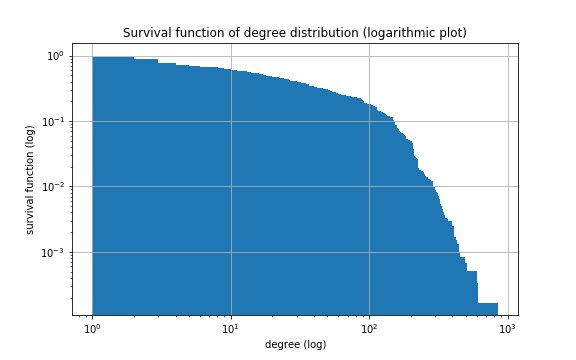
\includegraphics[width=.5\linewidth]{deg_distr_surv_log}
	\caption{Survival function of degree distribution}
	\label{fig:1_surv_log}
\end{figure}
\pagebreak

\subsection{Degree centrality}

The first and easier centrality index studied is the degree centrality. It is defined for node $i$ as
\begin{equation}
C_{deg}(i)=\frac{deg(i)}{\max_{j}  deg(j) }
\end{equation}
where $deg(i)$ is the degree of node $i$.\\
The measure is normalized dividing by the maximum degree, so that $0\leq C_{deg} \leq 1$.
The value of $C_{deg}$ for each node is depicted in \cref{fig:1_deg_centrality}.

\begin{figure} [!ht]
	\centering
	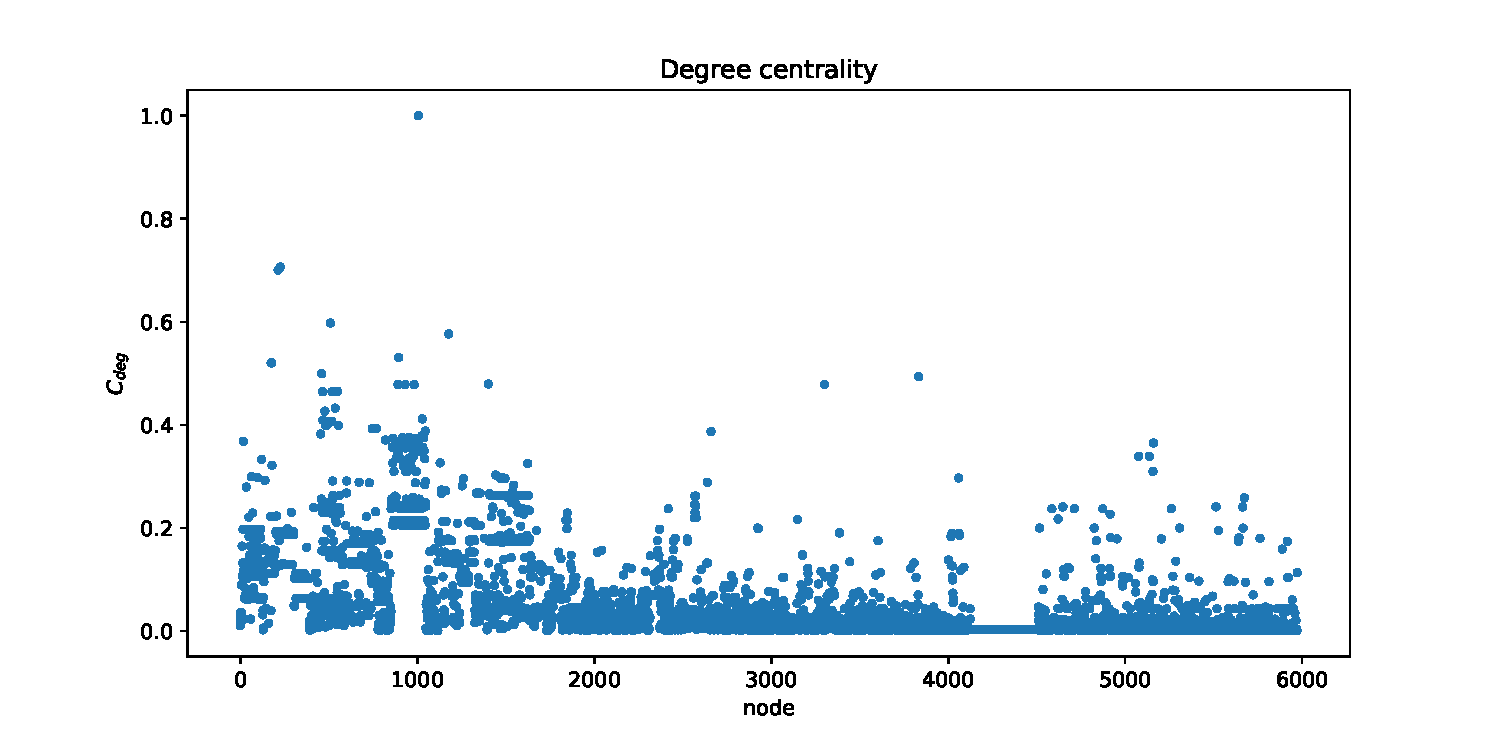
\includegraphics[width=.55\linewidth]{deg_centrality}
	\caption{Value of degree centrality for each node in the graph}
	\label{fig:1_deg_centrality}
\end{figure}

Even if very simple to compute, the degree centrality can give us useful indications of which node is more important in the network. Its limitation is that it only counts the number of adjacent nodes and doesn't exploit the structure of the graph.


\subsection{Katz centrality}
Katz centrality tries to assign an importance to each vertex according to the importance of its neighbours. This is an iterative process that at the end should converge to a final solution, which is the resulting centrality for every node. 
For a vertex $i$ in the graph, the Katz centrality is defined as
\begin{equation}\label{eq:1_katz}
x_i=\alpha \sum_{j}{A_{ij}x_{j}} + \beta_i
\end{equation}
where $A_{ij}$ is the adjacency matrix of the graph and $\beta_i=1$ to give an initial importance to all vertices.

To guarantee convergence the factor $\alpha$ is chosen such that $\alpha<1/\lambda_1$ with $\lambda_1$ largest eigenvalue of $A$.
For our network, $1/\lambda_1 \approx 0.004807$ and so we chose $\alpha=0.002$. $\lambda_1$ was calculated using numerical methods on sparse matrix.

The above \cref{eq:1_katz} can also be expressed in matrix form
\begin{equation}\label{eq:1_katz_mat}
\mathbf{x}=\alpha \mathbf{A} \mathbf{x} + \mathbf{1} \implies (\mathbf{I} - \alpha  \mathbf{A}) \mathbf{x}= \mathbf{1}
\end{equation}
and solved for $\mathbf{x}$ using specific solvers for sparse matrices, without expanding $\mathbf{A}$ to dense format.

The Katz centrality $C_{ka}$ (above was indicated as $\mathbf{x}$ for brevity) is calculated in both ways: with 1000 iterations of \cref{eq:1_katz} and by solving the system in \cref{eq:1_katz_mat}. With both methods, we obtained the same result up to approximation errors ($\approx 10^{-15}$). Fig. \ref{fig:1_katz_centrality} shows the value of $C_{ka}$ for each node.

\begin{figure} [!ht]
	\centering
	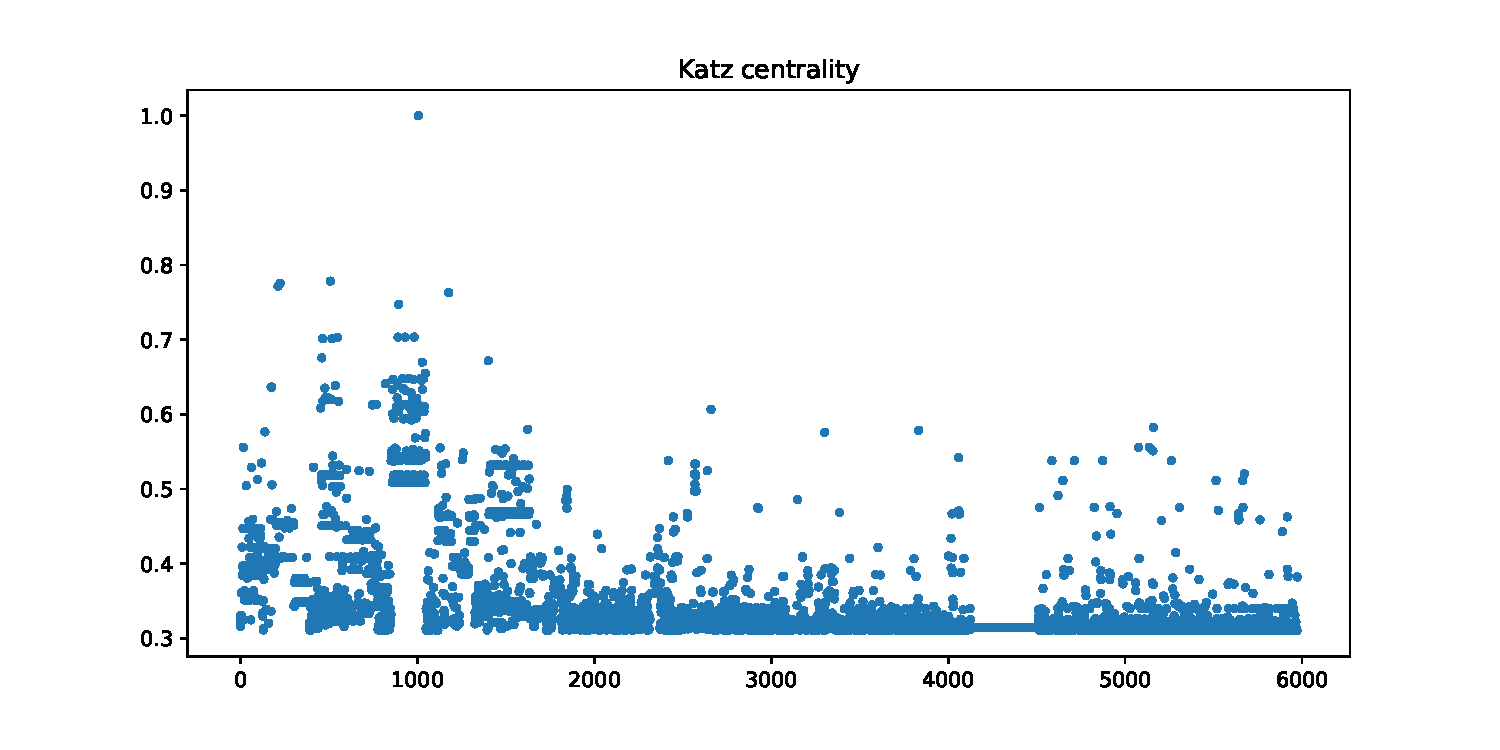
\includegraphics[width=.55\linewidth]{katz}
	\caption{Value of Katz centrality for each node in the graph}
	\label{fig:1_katz_centrality}
\end{figure}


\subsection{Betweenness centrality}

The last centrality considered is the betweenness centrality. It evaluates the importance of a node $i$ according to how many shortest paths pass through it. In particular,
\begin{equation}\label{eq:1_betw}
C_{betw}(i)= \sum_{s,t \neq i}{\frac{\sigma_i(s,t)}{\sigma(s,t)}}
\end{equation}
where $\sigma_i(s,t)$ is the number of shortest path from $s$ to $t$ passing through $i$ and  $\sigma(s,t)$ is the total number of shortest path from $s$ to $t$.\\
Notice that in case of parallel shortest paths, their effect on the centrality is split equally among them (we divide by their number $\sigma(s,t)$).

A simple algorithm to calculate betweenness centrality can be to compute all the shortest paths between any couple of nodes $(s,t)$ and count how many times these paths pass through node $i$, weighting by the number of shortest path from $s$ to $t$. This algorithm runs in $O(n^3)$, which can be too much for large networks.\\
A better solution for sparse graphs (as our case) is the Brandes' algorithm which runs in $O(n m)$. The basic idea is to perform an augmented BFS that keeps also the count of how many shortest paths are found. The graph is visited then in the reverse order to aggregate the results. A more detailed explanation of the algorithm is given in \cite{brandes_slides}, while the pseudocode, which we implemented in actual code, is available in the original paper \cite{brandes}.
In \cref{fig:1_between} the result of the algorithm on our graph is reported. The values are normalized so that $C_{betw} \in [0,1]$.

\begin{figure} [!ht]
	\centering
	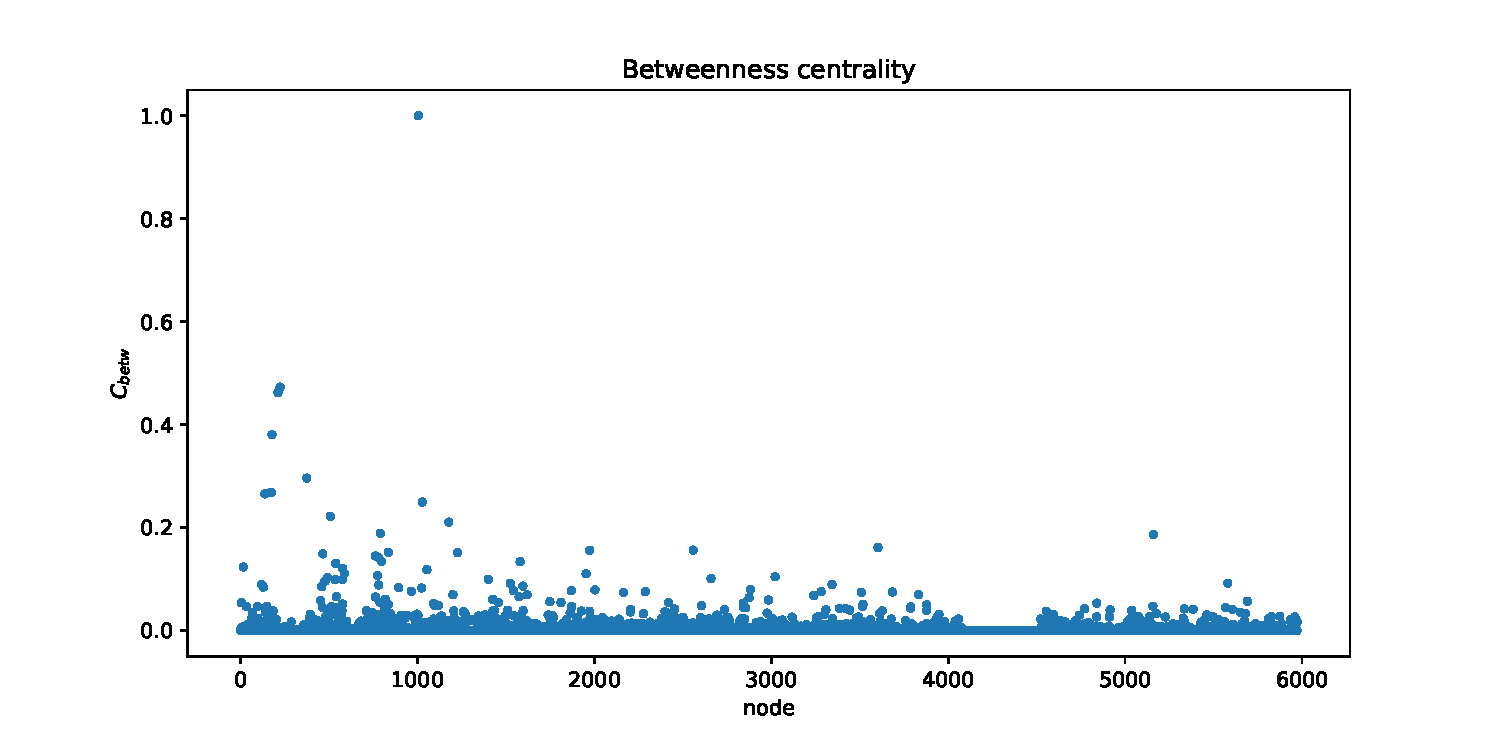
\includegraphics[width=.55\linewidth]{betweenness}
	\caption{Value of betweenness centrality for each node in the graph}
	\label{fig:1_between}
\end{figure}

\subsection{Final comparison and conclusions}
We can now draw a comparison among the different metrics considered. Degree, Katz and betweenness centralities for each node are plotted in \cref{fig:1_comparison_n}. Instead in \cref{fig:1_comparison_sort}, they are represented all sorted according to increasing Katz centrality.\\
We can notice that degree and Katz centrality are correlated and both follow the same trend. Betweenness centrality instead produces low values for most of the nodes (see also \cref{fig:1_between}), and peaks only for some of them, which are the central nodes in the networks where most of the paths pass. The different trend is due to the completely different way to compute the metric: betweenness looks for shortest paths in the whole network, while the others looks only to the adjacent nodes.
\\Interestingly, all the centralities assume value $1$ (maximum) for node $\#1006$. Therefore they all agree this is the most important node in the graph. 

In our case of protein-protein interaction graph, this indicates that $\#1006$ is the most important protein, which can be the focus to further studies and analyses by domain experts. But this result was obtained only by looking to the mathematical structure of the graph, without any labelling or knowledge about what the nodes represent. This proves the effectiveness of these methods, which can be applied in many different fields of science.

\begin{figure}[!ht]
	\centering
	\null\hfill
	\subfloat[for every node]{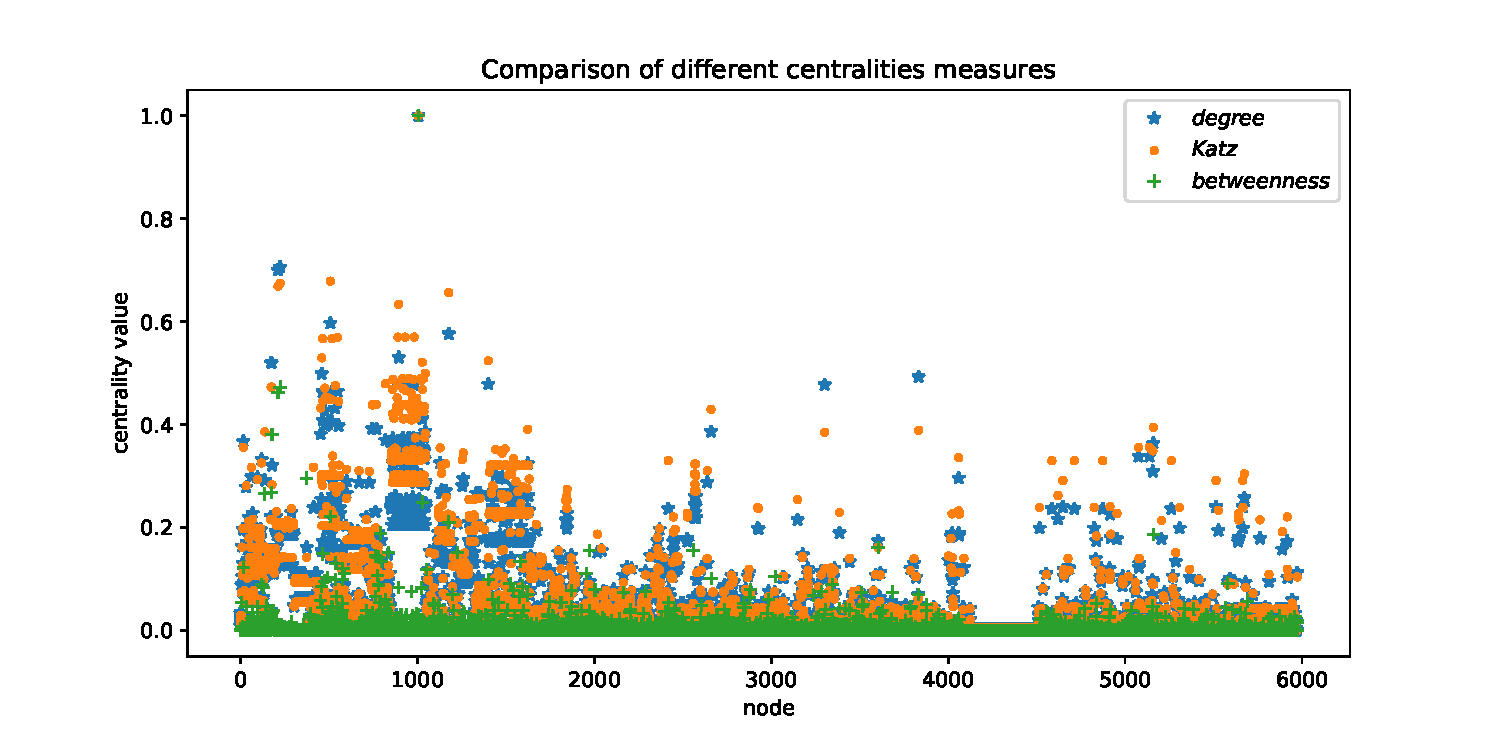
\includegraphics[width=.5\textwidth,clip, trim=0 0 0 0]{comparison}\label{fig:1_comparison_n}}
	\hfill
	\subfloat[sorted (increasing $C_{ka}$)]{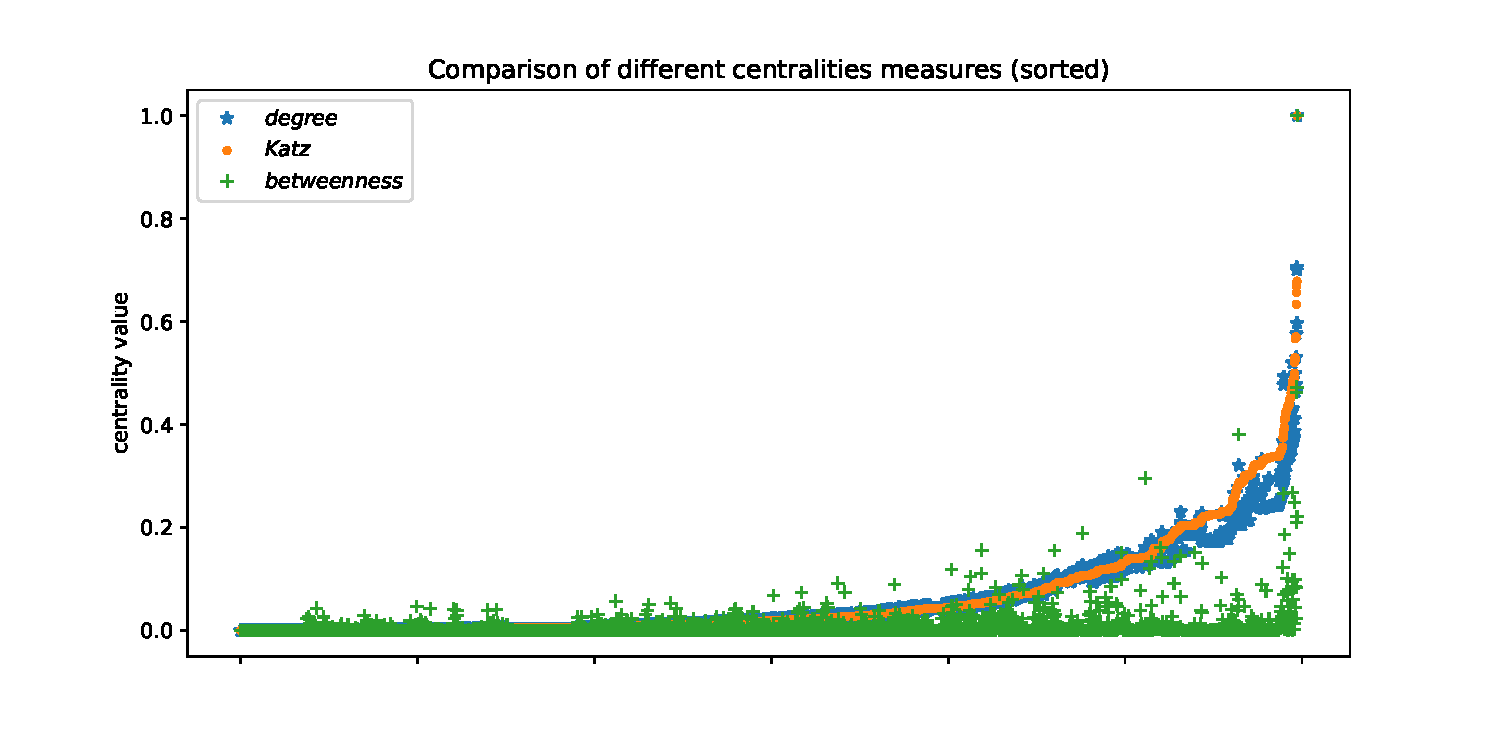
\includegraphics[width=.5\textwidth,clip, trim=0 0 0 0]{comparison_sort}\label{fig:1_comparison_sort}}
	\null\hfill
	\caption{Comparison of the different centralities indices}
	\label{fig:comparison}
\end{figure}
